TODO
- Adicionar pesquisa sobre paleta de cores e resultados

\mychapter{Metodologia}
\label{Cap:Metodologia}

Este capítulo aborda a metodologia aplicada no desenvolvimento do \textit{software}, quais métodos de engenharia de \textit{software} foram aplicados durante o processo, desde a concepção, até a prototipação

\section{Metodologia de Desenvolvimento do RADARE}

O desenvolvimento do \textit{software} RADARE adotou o método ágil Scrum como estrutura principal para orientar o processo de criação e entrega do produto \cite{softwareengreq}. Ele sendo uma metodologia ágil amplamente reconhecida, escolhido devido à sua capacidade de promover uma abordagem iterativa e flexível, especialmente adequada para uma equipe com um único desenvolvedor, como é o caso do desenvolvimento do RADARE \cite{scrum}.

\subsection{Descrição do método Scrum}

Scrum é uma metodologia ágil de desenvolvimento de \textit{software} que enfatiza a entrega iterativa e incremental de funcionalidades. Apesar de ter sido projetado para equipes multidisciplinares, pode ser adaptado para uma equipe de um só desenvolvedor devido aos seus princípios flexíveis e foco na entrega contínua de valor \cite{scrumlove}.
        
No Scrum, o trabalho é dividido em ciclos de desenvolvimento chamados de \textit{sprints}, geralmente com duração de duas a quatro semanas. Cada \textit{sprints} começa com uma reunião de planejamento, onde o desenvolvedor define as metas e prioridades do \textit{sprints} com base nas necessidades do projeto \cite{scrummic}. Durante o \textit{sprint}, o desenvolvedor trabalha na implementação das funcionalidades definidas no planejamento. O progresso é monitorado diariamente em reuniões curtas chamadas de \textit{daily scrums}, onde o desenvolvedor atualiza a equipe sobre o seu progresso, identifica quaisquer impedimentos e ajusta o plano conforme necessário. Ao final de cada \textit{sprint}, o desenvolvedor realiza uma revisão do \textit{sprint}, demonstrando as funcionalidades concluídas à equipe ou ao cliente, e uma retrospectiva do \textit{sprint}, identificando o que funcionou bem e o que pode ser melhorado no próximo \textit{sprint} \cite{scrumproj}.
        
Esse método de desenvolvimento de \textit{software} é funcional mesmo para equipes de um só desenvolvedor, promovendo uma abordagem colaborativa, adaptativa e transparente, permitindo que o desenvolvedor mantenha um alto nível de visibilidade e controle sobre o progresso do projeto. A abordagem iterativa e incremental do Scrum também facilita a adaptação a mudanças nos requisitos do projeto e permite que o desenvolvedor entregue continuamente valor de forma mais rápida e frequente ao cliente, ou orientador, no caso do RADARE \cite{scrum}.
        
\subsubsection{Aplicação do método Scrum no Desenvolvimento do \textit{Software} RADARE}

Ao utilizar o Scrum, o desenvolvedor pôde organizar o trabalho em ciclos curtos e mensuráveis, conhecidos como "\textit{sprint}". Cada \textit{sprint}, com duração definida, permite ao desenvolvedor focar em metas claras e alcançáveis, priorizadas com base nas necessidades do projeto. Essa abordagem iterativa possibilitou uma resposta rápida a mudanças nos requisitos e uma entrega contínua de funcionalidades ao longo do desenvolvimento.
        
Para o desenvolvimento do \textit{software} RADARE, o Scrum facilita a gestão eficiente do projeto, com reuniões diárias para monitorar o progresso, identificar possíveis obstáculos e ajustar o plano conforme necessário. Além disso, as reuniões de revisão de \textit{sprint} permitem uma demonstração transparente das funcionalidades desenvolvidas, garantindo uma comunicação eficaz com \textit{stakeholders} e a validação contínua do produto.
        
A aplicação do método Scrum no desenvolvimento do \textit{software} RADARE não apenas proporciona uma estrutura organizacional clara, mas também promove uma cultura de colaboração e melhoria contínua. Ao enfatizar a transparência, a comunicação e o \textit{feedback}, o Scrum permite ao desenvolvedor adaptar-se rapidamente às mudanças no ambiente de desenvolvimento e priorizar o valor entregue ao cliente.
        
Em resumo, a escolha do método Scrum para o desenvolvimento do \textit{software} RADARE demonstrou ser uma decisão acertada. Sua flexibilidade, foco na entrega de valor e capacidade de adaptação o tornaram uma escolha ideal para uma equipe de um único desenvolvedor, permitindo o desenvolvimento eficiente e eficaz de um produto de alta qualidade.
        
\section{Escopo do \textit{software}}

O escopo do projeto define os limites do trabalho a ser realizado, garantindo que todas as atividades estejam alinhadas com os objetivos do projeto. Isso proporciona uma base sólida para o planejamento, execução e controle do desenvolvimento do \textit{software}, permitindo que a concentração nas entregas essenciais para o projeto \cite{softwareeng}.

\subsection{Requisitos do Sistema}

Detalhe os requisitos funcionais e não funcionais do sistema de \textit{software}, identificados durante a fase de análise de requisitos. Explique como esses requisitos foram capturados e documentados \cite{softwareengreq}.
    
\subsubsection{Requisitos Funcionais}

Os requisitos funcionais no projeto de \textit{software} desempenham um papel crucial na definição das capacidades e funcionalidades que o sistema deve fornecer para atender às necessidades dos usuários. Em suma, eles representam o "o que" o sistema deve fazer. Esses requisitos são geralmente expressos em termos de casos de uso, cenários de interação do usuário ou fluxos de trabalho \cite{softwareengreq}.
        
A Tabela \ref{tab:req_funcional} demonstra os atuais requisitos funcionais do \textit{software}.

\begin{table}[htbp]
\begin{tabularx}{\linewidth}{|c|X|c|c|} \hline
\textbf{Identificador} & 
\textbf{Descrição} & 
\textbf{Prioridade} &
\textbf{Requisitos Relacionados}\\ \hline
RF01 & 
O sistema deve permitir que os usuários modelem a dinâmica dos sensores em uma planta industrial. & 
Alta & 
RF02 \\ \hline
RF02 & 
Os usuários devem ser capazes de alimentar o sistema com os dados gerados pelos sensores. & 
Alta & 
RF01 \\ \hline
\end{tabularx}

\caption{Tabela modelo dos requisitos funcionais.}
\label{tab:req_funcional}
\end{table}
            
% {\fontsize{10}{12}\selectfont \begin{longtable}
%     {| p{.15\textwidth} | p{.35\textwidth} | p{.20\textwidth} |  p{.20\textwidth} |} 
%     \hline
%     \textbf{Identificador} & \textbf{Descrição} & \textbf{Prioridade} & \textbf{Requisitos Relacionados} \\
%     \hline
%     RF01 & O sistema deve permitir que os usuários modelarem a dinâmica dos sensores presentes em uma planta industrial. & Alta & RF02 \\
%     \hline
%     RF02 & Os usuários devem ser capazes de alimentar o sistema com os dados gerados pelos sensores. & Alta & RF01 \\
%     \hline
%     RF03 & O sistema deve oferecer uma interface de usuário intuitiva e acessível. & Média & - \\
%     \hline
%     RF04 & O sistema deve realizar cálculos de reconciliação de dados de forma ágil e rápida. & Alta & RF01, RF02 \\
%     \hline
%     RF05 & O sistema deve garantir a compatibilidade de dados, mesmo com formatos heterogêneos. & Alta & RF01, RF02, RF03 \\
%     \hline
%     RF06 & Os usuários devem poder exportar os resultados da reconciliação de dados para diferentes formatos de arquivo. & Média & RF01, RF02, RF03, RF04, RF05 \\
%     \hline
%     RF07 & O sistema deve permitir aos usuários configurar alertas para notificar sobre eventos importantes relacionados aos dados dos sensores. & Alta & RF01, RF02 \\
%     \hline
%     RF08 & O sistema deve fornecer funcionalidades de visualização de dados em tempo real, incluindo gráficos e relatórios personalizáveis. & Alta & RF02, RF05 \\
%     \hline
%     RF09 & O sistema deve permitir a integração com outros sistemas de monitoramento industrial, facilitando a troca de dados e informações. & Alta & RF05, RF06 \\
%     \hline
% \caption{Tabela de Requisitos Funcionais} % needs to go inside longtable environment
% \label{tab:req_funcional}
% \end{longtable}}
        
\subsubsection{Requisitos Não Funcionais}

Os requisitos não funcionais em um projeto de \textit{software} desempenham um papel igualmente crucial, complementando os requisitos funcionais ao definir os critérios de qualidade, desempenho e restrições operacionais que o sistema deve atender. Enquanto os requisitos funcionais se concentram no "o que" o sistema deve fazer, os requisitos não funcionais delineiam "como" o sistema deve fazer isso, bem como outras características importantes que afetam sua operação e usabilidade e muitas vezes abordam características mais abstratas do sistema, como segurança, confiabilidade, escalabilidade, desempenho e usabilidade \cite{softwareengreq}. 
            
A Tabela \ref{tab:ReqNaoFuncional} demonstra os atuais requisitos não funcionais do \textit{software}.

{\fontsize{10}{12}\selectfont \begin{longtable}
{| p{.15\textwidth} | p{.45\textwidth} | p{.10\textwidth} |} 
    \hline
    \textbf{Identificador} & \textbf{Descrição} & \textbf{Prioridade} \\
    \hline
    RNF01 & O sistema deve ser altamente escalável para lidar com um grande volume de dados de sensores. & Alta \\
    \hline
    RNF02 & A segurança dos dados deve ser uma prioridade, garantindo proteção contra acesso não autorizado e manipulação indevida. & Alta \\
    \hline
    RNF03 & O desempenho do sistema deve ser otimizado para garantir tempos de resposta rápidos, mesmo em momentos de pico de uso. & Alta \\
    \hline
    RNF04 & O sistema deve ser facilmente configurável e customizável para atender às necessidades específicas de diferentes ambientes industriais. & Média \\
    \hline
    RNF05 & A manutenibilidade do sistema deve ser uma consideração fundamental, facilitando atualizações, correções de bugs e modificações futuras. & Média \\
    \hline
    RNF06 & A usabilidade do sistema deve ser intuitiva, permitindo uma curva de aprendizado mínima para os usuários. & Média \\
    \hline
    RNF07 & O sistema deve ser compatível com diferentes navegadores, garantindo sua acessibilidade em uma variedade de ambientes de implantação. & Alta \\
    \hline
    RNF8 & O sistema deve estar em conformidade com regulamentações de privacidade de dados, como GDPR, garantindo o tratamento adequado e a proteção das informações pessoais dos usuários. & Alta \\
    \hline
    RNF9 & A tolerância a falhas do sistema deve ser implementada, garantindo a continuidade das operações mesmo em caso de falhas de componentes individuais. & Alta \\
    \hline
    RNF10 & O tempo de resposta do sistema deve ser consistente e previsível, independentemente da carga de trabalho ou do número de usuários simultâneos. & Média \\
    \hline
\caption{Tabela de Requisitos Não Funcionais} % needs to go inside longtable environment
\label{tab:ReqNaoFuncional}
\end{longtable}}

\subsection{Temporização do Desenvolvimento do \textit{Software}}

O Gráfico de Gantt é uma ferramenta amplamente utilizada no gerenciamento de projetos para visualizar e acompanhar o progresso das atividades ao longo do tempo. Desenvolvido pelo engenheiro Henry Gantt na década de 1910, este gráfico fornece uma representação visual clara das tarefas do projeto, seus prazos e suas interdependências \cite{ganttchart}. 

Com sua disposição em forma de barras horizontais ao longo de um eixo de tempo, o gráfico permite que os gerentes de projeto e suas equipes identifiquem facilmente as datas de início e término de cada atividade, bem como as sobreposições e lacunas entre elas.
    
\begin{figure}[h]
    \centering
    \includegraphics[width=0.6\textwidth]{figuras/RADARE-Ganttt.pdf} % Replace "example.pdf" with the path to your PDF file
    \caption{Grafico de Gantt para desenvolvimento do \textit{software} RADARE.}
    \label{fig:ganttChart}
\end{figure}    

Na Figura \ref{fig:ganttChart} é visível Gráfico de Gantt utilizado pelo projeto, onde ele é separado nas seguintes partes: 
    
\begin{itemize}
    \item \textbf{Planejamento e Análise Inicial:} Esta fase inclui a identificação dos requisitos, definição dos objetivos, análise de viabilidade técnica e econômica, além da elaboração dos casos de uso e da documentação.
    
    \item \textbf{\textit{Design} e Prototipagem:} Nesta etapa, são criados o design de interface do usuário (UI) e o design de experiência do usuário (UX), bem como a definição da arquitetura do sistema e a prototipagem com revisões iterativas do design.
    
    \item \textbf{Desenvolvimento e Implementação:} Aqui ocorre a implementação do \textit{front} e \textit{back-end}, o desenvolvimento das funcionalidades principais do sistema, os testes unitários e a integração contínua, além da revisão e \textit{feedback} com os \textit{stakeholders}.
    
    \item \textbf{Testes e Garantia de Qualidade:} Esta fase abrange os testes de sistema abrangentes, a identificação e correção de \textit{bugs}, e a realização de testes de segurança para garantir a qualidade do sistema.
    
    \item \textbf{Preparação para Lançamento:} Envolve a preparação do ambiente de produção, o treinamento de usuários finais e o lançamento suave do sistema para garantir uma transição tranquila para os usuários.
    
    \item \textbf{Suporte e Manutenção Pós-Lançamento:} Por fim, inclui o monitoramento contínuo do sistema, atualizações regulares de \textit{software} e fornecimento de suporte técnico aos usuários para garantir o bom funcionamento e a satisfação contínua dos clientes.
\end{itemize}

Desta forma, a utilização do gráfico de Gantt foi crucial, por manter uma organização temporal da produção em razão do tempo decorrido, na qual auxiliou no planejamento e coordenação das diferentes etapas do projeto, permitindo também uma rápida avaliação do progresso do projeto, destacando visualmente as atividades concluídas, as em andamento e as pendentes. Auxiliando a identificar áreas de atraso ou potenciais gargalos, permitindo que a tomada de atitudes corretivas para manter o projeto no caminho certo.
        
\section{Projeto de \textit{Software}}

Descreva o processo de \textit{design} do \textit{software}, incluindo a arquitetura geral do sistema, diagramas de classe, diagramas de sequência, entre outros artefatos de \textit{design}. Explica as decisões de \textit{design} tomadas e como elas estão alinhadas com os requisitos do sistema \cite{softwareeng}.

\subsection{Arquitetura Geral do Sistema}

Durante o desenvolvimento de um \textit{software}, é crucial o uso de representações visuais para uma compreensão mais clara das funcionalidades e estrutura do projeto. Assim, a linguagem de modelagem unificada (UML) permite a criação de diversos tipos de diagramas para representar diferentes aspectos do sistema. Para a solução deste programa, optou-se pelo uso do PlantUML \cite{plantumldoc}, que possibilita a modelagem dos processos através de código, facilitando a alteração e atualização dos diagramas \cite{softwareengreq}.

\subsubsection{Diagrama de Classe}

O diagrama de classes é uma representação visual do projeto na engenharia de \textit{software}, empregada para descrever a estrutura estática de um sistema baseado em objetos \cite{softwareenguml}. Na sua forma mais básica, um diagrama de classes consiste em classes, que são os blocos de construção de um sistema orientado a objetos, contendo os atributos que as características ou propriedades dos objetos dessa classe, enquanto os métodos indicam as operações que podem ser realizadas por esses objetos, como é o caso do diagrama da Figura \ref{fig:ClassDiagram}. Essa estrutura fornece uma representação abstrata e organizada das entidades do sistema, permitindo uma compreensão clara de sua composição e funcionalidades.
            
\begin{figure}[htb]
    \caption{\label{fig:ClassDiagram}Diagrama de Classe em UML.}
    \begin{center}
        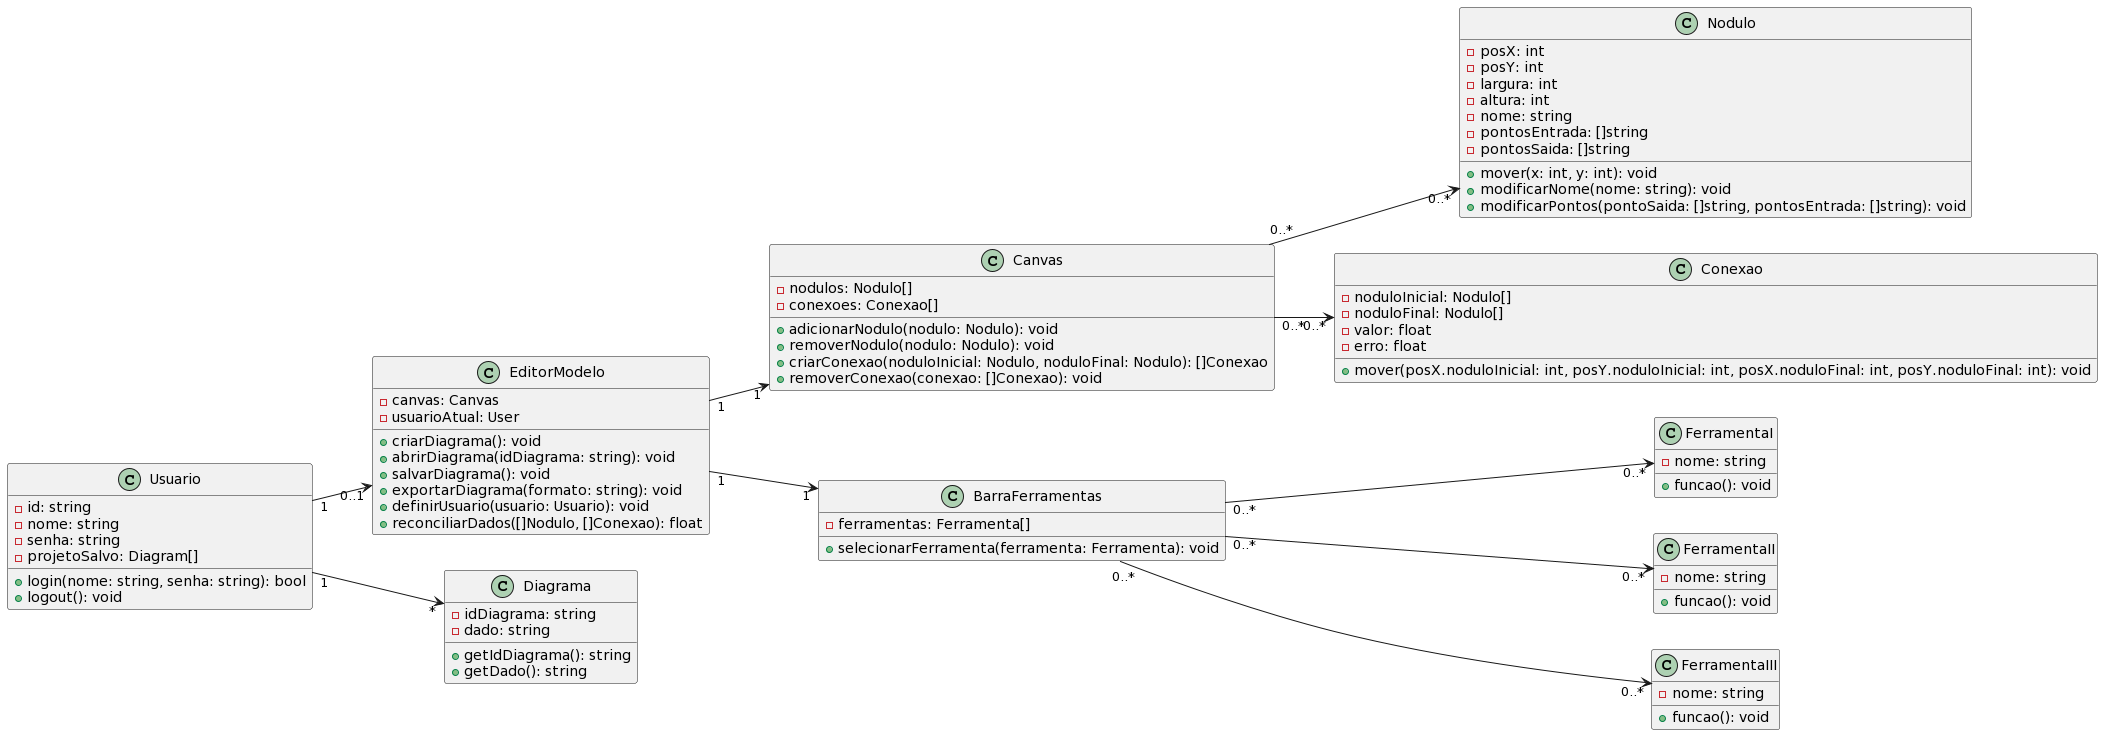
\includegraphics[width=0.6\textwidth]{figuras/ClassDiagram.png}
    \end{center}
\end{figure}
            
Adicionalmente, os relacionamentos entre as classes são destacados por meio de linhas que conectam os blocos das classes. Essas associações podem assumir diferentes formas, como associações simples, agregações, composições, heranças, entre outras, e fornecem \textit{insights} valiosos sobre como as diferentes partes do sistema interagem e dependem umas das outras.
            
Assim, um diagrama de classes torna-se uma ferramenta essencial para modelar a estrutura estática de um sistema, oferecendo uma representação visual nítida das classes, atributos, métodos e seus inter-relacionamentos, o que simplifica o processo de \textit{design}, análise e comunicação entre os integrantes da equipe de desenvolvimento de \textit{software} \cite{softwareenguml}.
            
\subsubsection{Diagrama de Caso de Uso}
        
O diagrama de caso de uso é uma representação visual amplamente utilizada na engenharia de \textit{software} para descrever a interação entre um sistema e seus usuários. Ele destaca os diferentes casos de uso, que representam as diferentes maneiras pelas quais os usuários interagem com o sistema para atingir seus objetivos. Na sua forma mais básica, um diagrama de caso de uso consiste em atores, que são os usuários externos ao sistema, e de casos de uso, que são as diferentes funcionalidades ou serviços oferecidos pelo sistema, como exemplificado no diagrama da Figura \ref{fig:UseCaseDiagram}.
        
\begin{figure}[htb]
    \caption{\label{fig:UseCaseDiagram}Diagrama de Caso de Uso em UML.}
    \begin{center}
        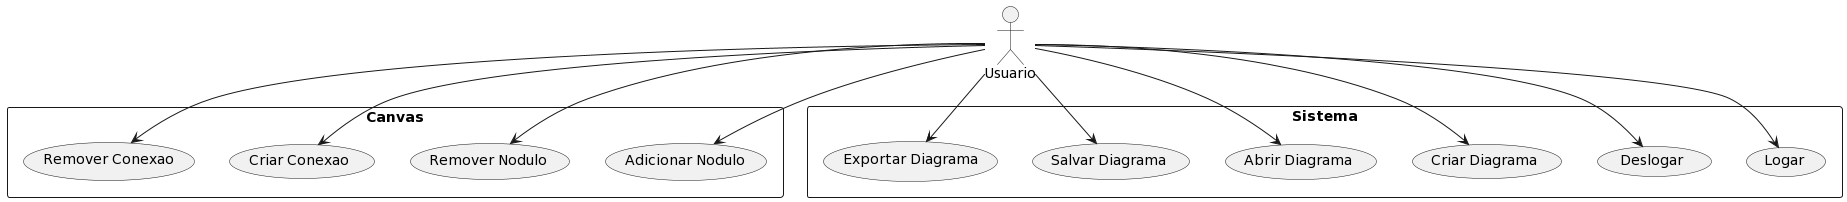
\includegraphics[width=0.6\textwidth]{figuras/UseCaseDiagram.png}
    \end{center}
\end{figure}
        
Os atores representam os diferentes tipos de usuários que interagem com o sistema, enquanto os casos de uso representam as diferentes funcionalidades oferecidas pelo sistema. Esses casos de uso são conectados aos atores por meio de linhas, indicando a interação entre os usuários e as funcionalidades do sistema.
        
Assim, um diagrama de caso de uso torna-se uma ferramenta essencial para modelar a interação entre um sistema e seus usuários, oferecendo uma representação visual clara dos atores, casos de uso e seus inter-relacionamentos. Isso simplifica o processo de \textit{design}, análise e comunicação entre os membros da equipe de desenvolvimento de \textit{software}, garantindo uma implementação eficaz e orientada às necessidades dos usuários.
        
\subsubsection{Diagrama do Banco de Dados}

O diagrama de banco de dados é uma representação visual das estruturas de dados e dos relacionamentos entre elas em um sistema de banco de dados \cite{databasedepth}, na qual visa representar a estrutura dos dados armazenados em um banco de dados e como esses dados estão relacionados entre si, como é o caso da Figura \ref{fig:DatabaseDiagram}, que representa o banco de dados do sistema.
            
\begin{figure}[htb]
    \caption{\label{fig:DatabaseDiagram}Diagrama de Banco de Dados em UML.}
    \begin{center}
        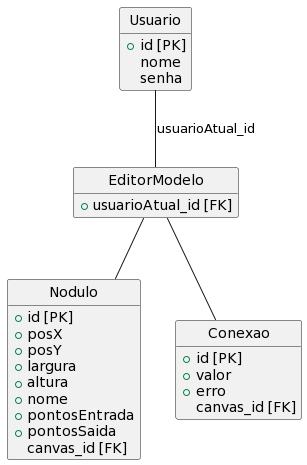
\includegraphics[width=0.6\textwidth]{figuras/DatabaseDiagram.png}
    \end{center}
\end{figure}
            
No diagrama de banco de dados, as entidades são representadas por tabelas, onde cada tabela possui colunas que representam os atributos dos dados armazenados. Além disso, as relações entre as tabelas são representadas por meio de chaves estrangeiras, indicando como os dados de uma tabela estão relacionados aos dados de outra tabela.
            
Desta forma, um diagrama de banco de dados é uma ferramenta vital para modelar a estrutura dos dados em um sistema de banco de dados, oferecendo uma representação visual clara das tabelas, colunas e relacionamentos entre elas. Isso facilita o projeto, análise e comunicação entre os membros da equipe de desenvolvimento de \textit{software}, garantindo uma implementação eficiente e eficaz do sistema de banco de dados.
    
\section{Implementação}

O projeto utilizou-se da ferramenta Node.js para gerenciamento de pacotes, permitindo uma gestão eficiente das dependências do projeto. Também foram empregados diversos \textit{plugins} e bibliotecas complementares para facilitar o desenvolvimento e melhorar a experiência do usuário.

O \textit{front-end} do projeto foi implementado utilizando React.js como a principal biblioteca de desenvolvimento de interfaces de usuário. Para estilização, foram empregados arquivos CSS com metodologia BEM (Block Element Modifier) para garantir uma estrutura de estilo escalável e modular. Além disso, o projeto se beneficiou do uso de diversos componentes reutilizáveis para manter um código limpo e organizado \cite{eloquentjavascript}.

Uma outra ferramenta muito utilizada, ainda no \textit{front-end} foi a biblioteca ReactFlow, de criação de diagramas, que foi adaptada para a solução em questão.
    
\section{Gerenciamento de Configuração e Mudança}

Durante o ciclo de vida do desenvolvimento de \textit{software}, foram adotadas diversas práticas e ferramentas para garantir um controle efetivo de versão e gerenciamento de mudanças \cite{gitevery}.
    
Para controle de versão, o Git foi escolhido como sistema de controle de versão distribuído. A plataforma Github \cite{github} foi utilizada para armazenar os repositórios do código-fonte do \textit{software}, o código LaTeX da Trabalho de Conclusão de Curso e da Apresentação. Isso permitiu que a existência de um histórico detalhado de todas as alterações realizadas no código.
    
Além disso, foram estabelecidas políticas de \textit{branches} no Git, como o uso de \textit{branches} de \textit{feature}, \textit{develop} e \textit{main}, para organizar o fluxo de trabalho e facilitar a integração contínua. As alterações no código eram revisadas antes de serem mescladas nos \textit{branches} principais, garantindo a qualidade e consistência do código.
    
Para o gerenciamento de mudanças, uma abordagem baseada em metodologias ágeis foi adotada, utilizando o Scrum. Isso permitiu que as mudanças fossem gerenciadas de forma iterativa e incremental, com entregas frequentes e \textit{feedback} contínuo ao orientador do trabalho.
    
Além disso, foi se utilizado o Trello como ferramenta de rastreamento de problemas \textit{(issue tracking)}, para registrar e acompanhar as mudanças, correções de \textit{bugs} e novas funcionalidades ao longo do desenvolvimento. Isso proporcionou uma visão clara do progresso do projeto e facilitou a comunicação dentro da equipe.
    
Desta forma, o controle de versão e gerenciamento de mudanças foram fundamentais para garantir a integridade, rastreabilidade e qualidade do \textit{software} ao longo de seu desenvolvimento, permitindo uma um comportamento eficaz da e uma entrega de progresso contínua no desenvolvimento do \textit{software}.